%% Generated from METHOD.md by scripts/md_to_latex.py - edit the Markdown, then re-run the script.
%% Compile with XeLaTeX or LuaLaTeX (e.g. tectonic METHOD.tex).
\documentclass[10pt,a4paper]{article}
\usepackage[margin=2cm]{geometry}
\usepackage{fontspec}
\setmainfont{DejaVuSerif.ttf}[BoldFont=DejaVuSerif-Bold.ttf, ItalicFont=DejaVuSerif-Italic.ttf,
  BoldItalicFont=DejaVuSerif-BoldItalic.ttf, Scale=0.92]
\setmonofont{DejaVuSansMono.ttf}[BoldFont=DejaVuSansMono-Bold.ttf, Scale=0.85]
\usepackage{graphicx,longtable,array,enumitem,fvextra,xcolor}
\usepackage[hidelinks]{hyperref}
\usepackage{xurl}
\setlist{nosep,leftmargin=1.4em}
\setlength{\parindent}{0pt}
\setlength{\parskip}{0.5em}
\renewcommand{\arraystretch}{1.2}
\begin{document}

{\LARGE\bfseries Cabin\_Noise: the paper pipeline\par}\bigskip

\textbf{Restructured 2026-11-02; audited the same day (AUDIT.md).} Every block follows a published low-fidelity method exactly and is verified against that paper's own equations. Nothing beyond the papers is in the pipeline.

\textbf{Sources:} \texttt{references/\allowbreak{}} (NASA NTRS, hashes in \texttt{references/\allowbreak{}SOURCES.\allowbreak{}md}) and \texttt{.\allowbreak{}.\allowbreak{}/\allowbreak{}PAIN\_\allowbreak{}Program/\allowbreak{}references/\allowbreak{}}.

\section*{1. The chain}

\begin{center}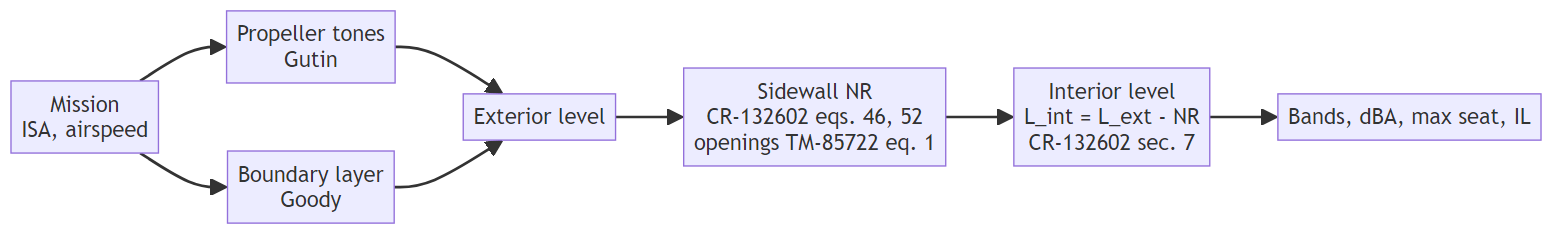
\includegraphics[width=\linewidth,height=0.3\textheight,keepaspectratio]{../figures/mermaid/METHOD-8cc90700eb.png}\end{center}

{\small
\begin{longtable}{>{\raggedright\arraybackslash}p{0.095\linewidth}>{\raggedright\arraybackslash}p{0.276\linewidth}>{\raggedright\arraybackslash}p{0.233\linewidth}>{\raggedright\arraybackslash}p{0.276\linewidth}}
\hline
\textbf{Block} & \textbf{Method, exactly} & \textbf{Source} & \textbf{Verified by: case (Validation tab) or unit test (\texttt{tests/\allowbreak{}})} \\
\hline
\endhead
Atmosphere, airspeed & ISA. Mission input: Mach, or KCAS converted with the subsonic pitot relations, q\_c = p0 [(1 + 0.2 (V\_c / a0)\textasciicircum{}2)\textasciicircum{}3.5 - 1], M = sqrt(5 [(q\_c / p + 1)\textasciicircum{}(2/7) - 1]). Flight-test runners (CR-178004): TAS = IAS sqrt(rho0 / rho) & US Std. Atm. 1976; standard pitot-static relations & unit tests \texttt{test\_\allowbreak{}isa\_\allowbreak{}against\_\allowbreak{}us\_\allowbreak{}standard\_\allowbreak{}atmosphere} (US Std. Atm. table), \texttt{test\_\allowbreak{}sutherland\_\allowbreak{}viscosity\_\allowbreak{}table\_\allowbreak{}value}, \texttt{test\_\allowbreak{}tas\_\allowbreak{}and\_\allowbreak{}measured\_\allowbreak{}temperature}, \texttt{test\_\allowbreak{}calibrated\_\allowbreak{}airspeed\_\allowbreak{}to\_\allowbreak{}mach} (sea level CAS = TAS; 250 KCAS at 25000 ft = 363 KTAS) \\
Propeller tones & Gutin: p\_m = (mB Omega / 2 sqrt2 pi c r) abs(T cos(theta) - Q c / (Omega R\_e\textasciicircum{}2)) J\_mB(...), R\_e = 0.8 R\_t, at the fuselage point nearest the propeller; one propeller per side, sides in energy & Gutin 1936; NASA RP-1258 vol. 1 ch. 1 & case V0a: direct quadrature of the dipole integral (1e-12 dB); unit test \texttt{test\_\allowbreak{}gutin\_\allowbreak{}against\_\allowbreak{}direct\_\allowbreak{}time\_\allowbreak{}domain\_\allowbreak{}moving\_\allowbreak{}force\_\allowbreak{}far\_\allowbreak{}field} (0.1 dB) \\
Boundary layer & Goody wall spectrum on a 1/7-power flat-plate layer; diffuse equivalent <p\textasciicircum{}2> = <p\_wall\textasciicircum{}2> / 2 & Goody 2004; Schlichting; Waterhouse 1955, CR-3813 p. 23 & unit tests \texttt{test\_\allowbreak{}goody\_\allowbreak{}asymptotic\_\allowbreak{}slopes\_\allowbreak{}and\_\allowbreak{}flat\_\allowbreak{}plate\_\allowbreak{}layer} (Goody's +2 / -5 slopes; delta and Cf of the 1/7-power law) and \texttt{test\_\allowbreak{}waterhouse\_\allowbreak{}wall\_\allowbreak{}factor\_\allowbreak{}and\_\allowbreak{}diffuse\_\allowbreak{}intensity} (Monte Carlo of the wall = 2 x diffuse factor). No V case: Goody gives no closed form to compare with \\
Wall transmission & random-incidence mass law, eq. (46) & NASA CR-132602 sec. 5.1 & case V1: eq. (46) = 0-90 deg integral of eq. (45) (1e-9) \\
Sidewall NR & non-resonant double wall, eq. (52): NR = 10 log[(1 + 4 alpha3 / (eps tau31))(1 + alpha5 / tau35) + alpha5 / tau31]; blanket mass on the trim (sec. 6.2); single wall: 10 log(1 + alpha5 / tau) & NASA CR-132602 sec. 5.2 & case V2: eq. (52) = numeric solution of the power balance eq. (47) (1e-14); case V2p: the report's Fig. 14 prediction (check failed, 3.3 dB); unit tests \texttt{test\_\allowbreak{}pipeline\_\allowbreak{}noise\_\allowbreak{}reduction\_\allowbreak{}is\_\allowbreak{}eq52\_\allowbreak{}and\_\allowbreak{}the\_\allowbreak{}single\_\allowbreak{}wall\_\allowbreak{}form}, \texttt{test\_\allowbreak{}double\_\allowbreak{}wall\_\allowbreak{}limits} \\
Openings & area-weighted transmission; double window = one pane of the summed mass; areas given per side, scaled with the exposed area & NASA TM-85722 eq. (1), p. 17 & unit tests \texttt{test\_\allowbreak{}openings\_\allowbreak{}combine\_\allowbreak{}by\_\allowbreak{}area\_\allowbreak{}as\_\allowbreak{}tm85722\_\allowbreak{}eq1} (eq. 1 written out), \texttt{test\_\allowbreak{}openings\_\allowbreak{}scale\_\allowbreak{}with\_\allowbreak{}the\_\allowbreak{}exposed\_\allowbreak{}area}. No V case: eq. 1 is an area average, so a case would repeat the unit test \\
Cabin & alpha5 S = A = sum S alpha (Sabine), or 0.161 V / T60 from measured T60 & Sabine; CR-132602 eq. (37) & unit tests \texttt{test\_\allowbreak{}cabin\_\allowbreak{}absorption\_\allowbreak{}is\_\allowbreak{}sabine} (sum S alpha by hand; measured-T60 path against 24 ln10 V / c T60), \texttt{test\_\allowbreak{}sabine\_\allowbreak{}constant}. No V case \\
Insertion loss & L\_bare - L\_treated = dTL + dABS & NASA TM-85722 eqs. (1)-(3) & case V3: within 0.28 dB (the "1 +" term of the single-wall form); unit tests \texttt{test\_\allowbreak{}identical\_\allowbreak{}configs\_\allowbreak{}have\_\allowbreak{}zero\_\allowbreak{}il}, \texttt{test\_\allowbreak{}heavier\_\allowbreak{}trim\_\allowbreak{}and\_\allowbreak{}more\_\allowbreak{}absorption\_\allowbreak{}give\_\allowbreak{}positive\_\allowbreak{}il} \\
Seat spread & P-th percentile seat = room average + 10 log10(ln(1 / (1 - P))); P an input, default 95 \% (+ 10 log10(ln 20) = 4.77 dB) & Schroeder 1962 & unit tests \texttt{test\_\allowbreak{}seat\_\allowbreak{}statistic\_\allowbreak{}is\_\allowbreak{}the\_\allowbreak{}exponential\_\allowbreak{}95th\_\allowbreak{}percentile}, \texttt{test\_\allowbreak{}seat\_\allowbreak{}percentile\_\allowbreak{}is\_\allowbreak{}the\_\allowbreak{}exponential\_\allowbreak{}quantile} (80-99 \%; quantiles of an exponential sample), \texttt{test\_\allowbreak{}pipeline\_\allowbreak{}uses\_\allowbreak{}the\_\allowbreak{}seat\_\allowbreak{}percentile}. No V case \\
Weighting & IEC A / C & IEC 61672-1 & unit test \texttt{test\_\allowbreak{}weighting\_\allowbreak{}against\_\allowbreak{}iec\_\allowbreak{}61672\_\allowbreak{}table} (A and C at 31.5 Hz-8 kHz, 0.1 dB). No V case \\
\hline
\end{longtable}}

\textbf{Cases and unit tests.} A V case is a check shown on the Validation tab, with a figure. A block whose paper gives nothing to compare a curve with (a table, a constant, an area average, a statistic) is verified by unit tests instead. They run with \texttt{pytest} (\texttt{tests/\allowbreak{}test\_\allowbreak{}sources.\allowbreak{}py}, \texttt{test\_\allowbreak{}methods.\allowbreak{}py}, \texttt{test\_\allowbreak{}pipeline.\allowbreak{}py}, \texttt{test\_\allowbreak{}inputs.\allowbreak{}py}) and are as binding: a failing test blocks a change. Each unit test compares the code with a published table, an independent derivation or a hand calculation, never with itself. Measured-data validation of the blocks together is V4-V7 (sec. 4).

The end-to-end hand check (\texttt{tests/\allowbreak{}test\_\allowbreak{}end\_\allowbreak{}to\_\allowbreak{}end.\allowbreak{}py}) recomputes a tone and a band of the default case from these formulas, written out independently; the tool agrees within 0.01-0.05 dB.

\section*{2. Things found in the sources}

\begin{itemize}
\item \textbf{CR-132602 eq. (53) misprint.} It shows 2/eps; eq. (52) and the report's power balance give 4/eps. The numeric solution of eq. (47) confirms 4/eps, which is used.
\item \textbf{CR-132602's own limit.} Sec. 6.2 and 8(d) say the non-resonant model is invalid well below about half the ring frequency, where panel stiffness dominates. Propeller tones on small aircraft lie there.
\item \textbf{CR-132602 Fig. 14 (case V2p, 2026-11-02).} This is the paper's own printed NR prediction. Built from the inputs the report states, the code's single wall comes out 2.1-3.3 dB low, with the right shape.
\begin{itemize}
\item The report says it used eq. (53), whose area ratio S5/S2 it does not give. A post-hoc S5/S2 = 2 matches within 0.3 dB. The pipeline itself carries the ratio through A / S.
\item The double-wall curve also needs the unstated blanket mass, so it cannot settle 2/eps against 4/eps.
\end{itemize}
\item \textbf{Gutin is a far-field formula.} Applying it at the fuselage, which is in the near field, is the classic low-fidelity practice and is its known limit.
\end{itemize}

\section*{3. What was removed (2026-11-02)}

These were removed because they are not in the papers. Their code and validation records are in git, up to commit 1c2c8fe:

\begin{itemize}
\item the plane-wave transfer-matrix sidewall and its Delany-Bazley, limp and table blanket models;
\item the stiffened-bay stiffness;
\item the blade-geometry (BEMT) source and the moving-force near-field source;
\item cylinder scattering;
\item the patch grid and measured-level anchoring;
\item box-mode seat shapes and the twin coherent synchrophase sum.
\end{itemize}

Retired cases: V0b, V0c, V4c, V4d, V5d.

\section*{4. Validation of the paper pipeline (2026-11-02)}

Cases are defined in commit 93bbeb9, before the runs. The data were seen with the retired pipeline, so these runs are not blind; no parameter is chosen from the data. Criteria are unchanged (low-fi policy: at least 75 \% of points within +-6 dB; V4a: max error 3 dB).

{\small
\begin{longtable}{>{\raggedright\arraybackslash}p{0.049\linewidth}>{\raggedright\arraybackslash}p{0.430\linewidth}>{\raggedright\arraybackslash}p{0.430\linewidth}}
\hline
\textbf{Case} & \textbf{Data} & \textbf{Result} \\
\hline
\endhead
V5b & CR-178004 exterior boundary-layer bands & \textbf{met}, 82 \% \\
V6 & CR-178004 fiberglass insertion loss & not met, 72 \% (mean +1.4 dB) \\
V5 & CR-178004 exterior tones (Gutin + 6 dB flush doubling) & not met, 64 \% (mean -3.3 dB) \\
V4 & TM-85722 Fig. 18, lab TL of the prop-plane treated panel (run 2026-11-03) & not met, 5/11 bands; within 3 dB to 250 Hz, 6-13 dB low above 315 Hz (a single limp wall has no double-wall rise) \\
V4b & CR-3813 trimmed cylinder reverberant NR & not met, 26 \% \\
V5c & Report 996 static tones at d/D = 0.083 (Gutin) & not met, 29 \%; Gutin's far-field form at the blade tip \\
V4a & TP-1964 bare cylinder reverberant NR & not met, max 16.5 dB \\
V7 & CR-178004 cabin tones from the measured exterior & not met, 1 \%, +17.9 dB; mass-law wall far below 0.5 f\_r (the paper's stated limit) \\
\hline
\end{longtable}}

The misses are where the papers' own stated limits put them:

\begin{itemize}
\item at low frequency, below about 0.5 f\_r, for tones through a real fuselage;
\item in the near field for Gutin.
\end{itemize}

\section*{5. Inputs and fixed constants (2026-11-03)}

\textbf{Inputs.} Every input is a field of the project, and all of them can be edited in the GUI:

\begin{itemize}
\item Mission, Propeller, Fuselage, Sidewall, Openings and Cabin tabs;
\item the Analysis tab: band range and the max-seat percentile.
\end{itemize}

The default example's values are all in \texttt{cabin\_\allowbreak{}noise/\allowbreak{}data/\allowbreak{}default\_\allowbreak{}project.\allowbreak{}json}; none is set in code. Two tests enforce this (\texttt{tests/\allowbreak{}test\_\allowbreak{}inputs.\allowbreak{}py}):

\begin{itemize}
\item every field must appear in that file;
\item every field must have a GUI editor.
\end{itemize}

\textbf{Fixed constants.} These belong to the published equations. They are not inputs, so they cannot be changed by accident:

{\small
\begin{longtable}{>{\raggedright\arraybackslash}p{0.227\linewidth}>{\raggedright\arraybackslash}p{0.274\linewidth}>{\raggedright\arraybackslash}p{0.181\linewidth}>{\raggedright\arraybackslash}p{0.198\linewidth}}
\hline
\textbf{Constant} & \textbf{Value} & \textbf{Where} & \textbf{Source} \\
\hline
\endhead
Diffuse-field wall factor & wall p\textasciicircum{}2 = 2 x diffuse p\textasciicircum{}2 (3.0 dB) & \texttt{pipeline.\allowbreak{}WATERHOUSE\_\allowbreak{}DB} & Waterhouse 1955; CR-3813 p. 23 \\
Flat-plate turbulent boundary layer & delta = 0.37 x Re\textasciicircum{}-0.2, Cf = 0.0592 Re\textasciicircum{}-0.2 & \texttt{source\_\allowbreak{}tbl.\allowbreak{}boundary\_\allowbreak{}layer} & 1/7-power law, Schlichting \\
Goody spectrum & 3.0, 0.75, 0.5, 3.7, 1.1, -0.57, 7 & \texttt{source\_\allowbreak{}tbl.\allowbreak{}goody\_\allowbreak{}phi} & Goody 2004 \\
Gutin & 2 sqrt2 pi, Bessel J\_mB & \texttt{source\_\allowbreak{}tonal.\allowbreak{}gutin\_\allowbreak{}rms} & RP-1258 ch. 1 \\
Mass law & random incidence 0-90 deg, eq. (46) & \texttt{sea.\allowbreak{}tau\_\allowbreak{}mass\_\allowbreak{}law\_\allowbreak{}diffuse} & CR-132602 \\
Cavity epsilon & pi below c / 2L, 4 above & \texttt{sea} & CR-132602 eqs. (51)-(52) \\
Sabine & 0.161 V / A & \texttt{cabin.\allowbreak{}t60} & Sabine \\
Schroeder frequency & 2000 sqrt(T60 / V) & \texttt{cabin.\allowbreak{}schroeder\_\allowbreak{}frequency} & Schroeder 1962 \\
Seat statistic & 10 log10(ln(1 / (1 - P))) & \texttt{cabin.\allowbreak{}seat\_\allowbreak{}stat\_\allowbreak{}db} & Schroeder 1962 (P is an input) \\
ISA, Sutherland & US Std. Atm. 1976 & \texttt{atmosphere} &  \\
A / C weighting & IEC 61672-1 & \texttt{weighting} &  \\
Reference pressure & 20 uPa & \texttt{weighting.\allowbreak{}P\_\allowbreak{}REF} &  \\
\hline
\end{longtable}}

\end{document}
